\chapter{基于LSTM-CRF的中文序列标注模型}
\label{chap:3}
\section{引言}
由于基于统计的方法是在一定的假设前提下对自然语言进行建模,其复杂程度远远不能与灵活多变的自然语言相比,且大多数基于统计的模型若想取得较好的识别效果,总要较大程度地依赖人工构建语料库、字典、特征等手段,且不同语言、不同领域语料之间模型的可迁移性也较差,这在一定程度上限制了基于统计的模型在自然语言处理中进一步的应用。

早在上世纪80年代,神经网络就作为机器学习领域的一个重要的研究方向受到关注。
人工神经网络可以定义为“由具有适应性的简单单元组成的广泛并行互联的网络,它的组织能够模拟生物神经系统对真实世界的物体作出的交互反应”。
其中,这个“具有适应性的简单单元”来源于1943年McCulloch和Pitts提出的M-P神经元模型。
这一模型实际上就是对生物学意义上的神经元进行的一种形式化的数学描述。
早期的神经网络结构较为简单,受到硬件计算能力的限制,一般层数较少,多用于简单模型中;由于结构复杂的网络在训练中存在严重的过拟合问题,且训练效率很低,导致神经网络的发展陷入低谷。
\citet{hinton2009deep}在2006年提出深度学习的概念,指出深层神经网络可以通过组合低层特征获得能够更好地体现数据特性的高层特征,这些特征能够更好地对数据的本质信息进行整合抽象地刻画。
同时还提出了基于深度置信网络的非监督贪心逐层训练算法,能够较好地适应深层网络结构,解决了当网络层数较多时的训练难的问题。

深度学习方法在多个领域都有着重要的应用。
\citet{lecun1998gradient}提出的卷积神经网络(CNN)在图像识别领域得到了广泛应用。
\citet{krizhevsky2012imagenet}等人在2012年将CNN应用于ImageNet数据集上,取得了图像分类和目标定位的最佳结果。
此后CNN在各项任务中都大显身手,在人脸识别、视频分类、行为识别等方向上都取得了较好的效果。

而对于以序列信号作为输入的问题,如语音识别、机器翻译和序列标注等方向,循环神经网络(RNN)则成为了解决这类问题的主要手段。
这其中又以能够较好地获取较长距离内上下文依赖的长短时记忆网络(LSTM)最为突出。

本章针对命名实体识别问题,从几个方面对实现实体识别的基于LSTM-CRF的中文序列标注框架进行介绍。
本章将对词的分布式表示进行介绍,考察循环神经网络的基本结构,对比分析长短时记忆网络及其各种变体的实现,最后在一个具体的命名实体识别任务场景下,构建基于LSTM-CRF的序列标注框架,并给出针对该任务命名实体的额外字符级特征的改进方法,最后设计实验验证改进方法的有效性。

\section{词的分布式表示}
\subsection{从统计语言模型到神经网络语言模型}
不论是传统的基于统计的方法还是基于神经网络的方法,进行命名实体识别任务首先要将自然语言词汇转化为模型能够处理的形式,即实值向量。
最基本的词的向量化表示就是one-hot representation,其形式为一个维度为词表大小的$\{0, 1\}$向量,设该词在词表中的索引为$i$,则其one-hot向量只在位置$i$上的值为1,其余位置为0。
这种表示方法有很多缺陷,首先不同的词并不能从其对应的one-hot向量中判别其语义相关程度,它基本不包含词汇的语义信息;其次,获取one-hot向量仅仅通过建立词表即可实现,忽略了词汇的上下文特征而完全将词独立对待;最后,这种向量的维度为词典大小,显然非常稀疏,在深度神经网络模型中非常容易导致维数灾难。

\begin{figure}[H]
    \centering
    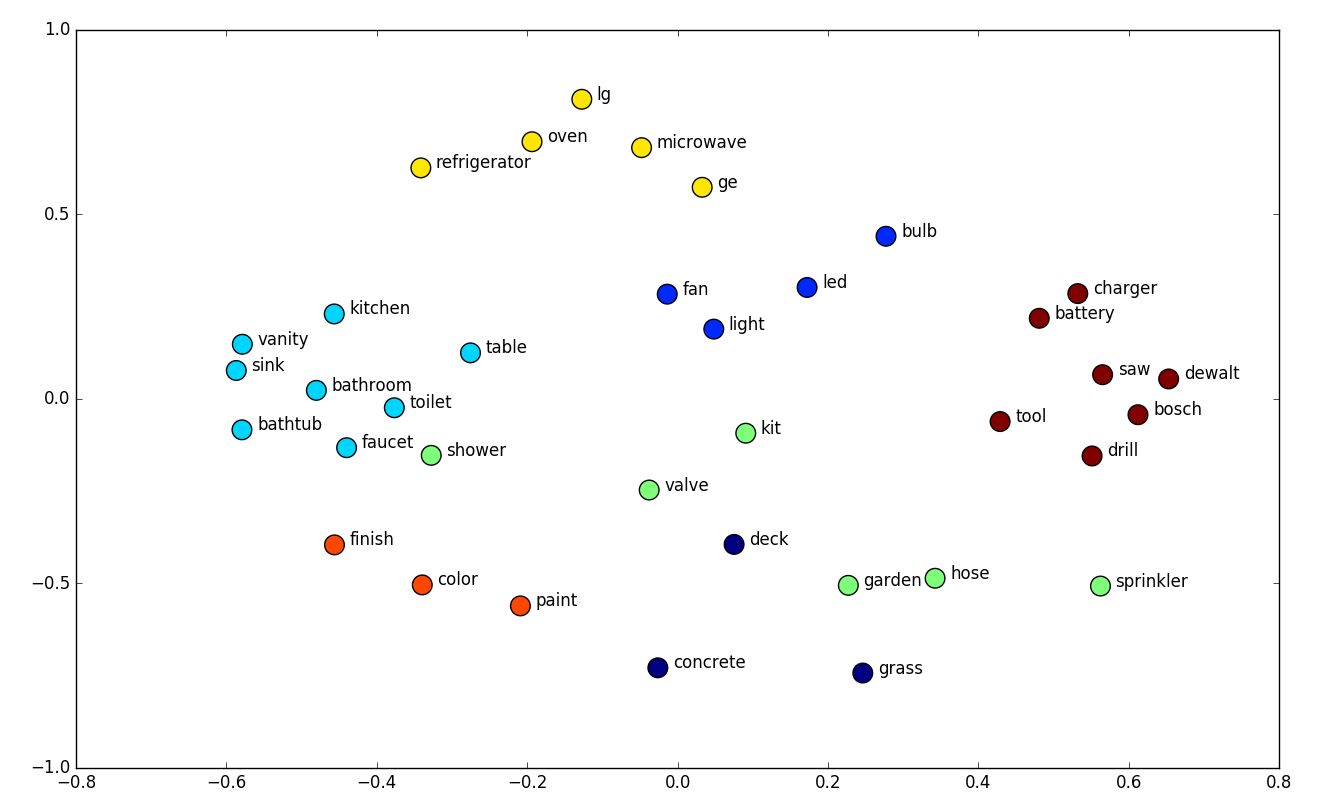
\includegraphics[width=\textwidth]{word_embedding.png}
    \bicaption{词嵌入将词映射到高维空间中的点}{Word embeddings projects words to points in high dimension space}
    \label{fig:word_embedding}
\end{figure}

词的分布式表示最初由Hinton\citep{hinton1986distributed, hinton1986learning}于1986年提出。
与one-hot representation不同的是,分布式表示下的词向量维度不再是词表大小,而是一个相对较低的固定维度。其中的每一个分量也不再是0或者1,而是一个实值。
这时词汇表可以视作是一个向量空间,词即是空间中的点。
既然是空间,就可以定义距离,这个距离可以理解为词汇在语义或语法层面上的距离。
如图\ref{fig:word_embedding}所示,这样词与词之间就不是孤立的了,词在上下文中的语义信息也得到了保留,词向量维度人为可控且远远小于词表大小。

估计词向量参数的方法有很多种,包括隐含语义分析(latent semantic analysis, LSA)、隐狄利克雷分布(latent Dirichlet allocation)和利用神经网络的方法。

Bengio等人在2003年提出了基于神经概率的语言模型。利用神经网络估计语言模型参数的同时,得到了作为副产品的词向量。
其基本的思路是,首先赋予每个词一个词特征向量$\Vector{v}(\Vector{v}\in \Set{R}^m)$,$m$为可以设定的词向量维度,如50,100,200等;然后使用这些词特征向量来表示一段文本序列的联合概率函数:
最后在训练过程中,同时更新(学习)词特征向量和概率函数的参数(语言模型参数)。

在章节2.1.1中介绍了n元语言模型。语言模型的目标是计算给定序列在该语言下的概率,这个概率通过一系列条件概率的乘积表示:
\begin{equation}
    P(w^T_1) = \prod^{T}_{t=1}P(w_t|w_1^{t-1})
\end{equation}
其中$T$为序列长度,$w_i^j = (w_i, w_{i+1},\dots, w_j)$。但由于这种计算方式参数过多,后来模型可以简化为序列某时刻词的条件概率只依赖其上文的若干个词(n-gram):
\begin{equation}
    P(w_t|w_1^{t-1}) \approx P(w_t|w^{t-1}_{t-n+1})
\end{equation}
通过统计各词序列出现的次数作为条件概率值,填充训练模型参数。

另一种估计模型参数的方法是对模型建立一个目标函数,将参数训练转化为对一个关于模型参数和训练数据的函数优化问题。
实际中,常使用最大对数似然函数作为目标函数,通过调整其参数获得对数似然函数的最大值,此时得到的就是较为理想的参数。
\begin{equation}
    \mathcal{L} = \sum_{c\in C} \log p(w|Context(w))
\end{equation}
在语言模型中,关于某时刻词$w$上下文的条件概率可以用$Context(w)$表示。于是其中的条件概率就可以表示为关于词和其上下文的$Context(w)$的函数:
\begin{equation}
    p(w|Context(w)) = F(w, Context(w), \theta)
\end{equation}
其中$\theta$就是待训练参数集。

在神经语言模型中,获取关于词以其上文为条件的条件概率
\begin{equation}
    f(w_t, \dots, w_{t-n+1}) = P(w_t|w_1^{t-1})
\end{equation}
被分解为两部分,其一是将词表$V$中的词映射为实值向量的矩阵$\Matrix{C}$,其维度是$|V|\times m$;
其二是获得条件概率的映射函数$g$,该函数接受序列$w_{t-n+1}^{t-1}$在实值矩阵$C$中的对应各行向量作为输入,输出给定序列下$w_t$是词典中某个词的概率分布。
于是上面的函数$f$可以进一步表示为:
\begin{equation}
    f(i, w_{t-1}, \dots, w_{t-n+1}) = g(i, C(w_{t-1}), \dots, C(w_{t-n+1}))
\end{equation}

在具体的操作上,模型采用了一个三层神经网络进行参数学习,结构包括输入层、隐藏层和输出层。
值得注意的是其输入层进行的操作是将词$w$上文$n-1$个词的词向量首尾相连得到特征向量$x_w$输入到隐层中。
网络使用传统的前后向传播方法进行参数学习,与其他模型不同的是,在后向传播的最后一步,通过计算${\partial\mathcal{L}}/{\partial x}$并取其中相应维度的部分,实现了一次训练之后批量更新作为输入的$n-1$个词向量的过程。

\subsection{Word2Vector基本原理}
在Bengio工作的基础上,谷歌的Tomas Mikolov团队实现了开源工具word2vec,其中使用了两个模型:CBOW(continous bag of word)模型和Skip-gram模型。
\begin{figure}[H]
    \centering
    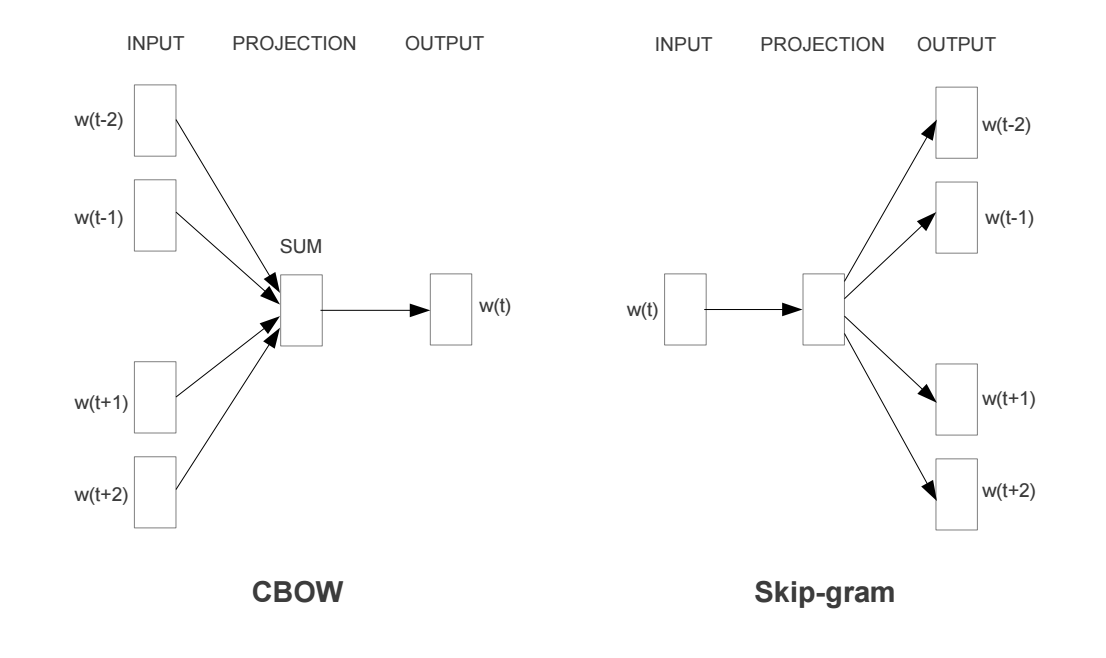
\includegraphics[width=\textwidth]{w2v.png}
    \bicaption{CBOW与Skip-gram模型示意图}{CBOW and Skip-gram model}
    \label{fig:w2v}
\end{figure}
与之前提到的根据上文预测下一个词不同的是,CBOW通过设置一个固定大小的上下文窗口$c$,如设置为2,利用$w_{t-2}, w_{t-1}, w_{t+1}, w_{t+2}$预测当前词$w_t$,Skip-gram则是通过当前词$w_t$预测其上下文。其结构如图\ref{fig:w2v}所示。
神经网络模型将上文词向量连接作为隐层输入,隐层中的激活函数为\verb|tanh|。
CBOW同样使用三层的神经网络结构,包括输入层、投影层和输出层,但投影层的输出是通过窗口内$2c$个词向量的和构建的。
并且CBOW模型中并不存在隐藏层,也就没有激活函数。
最后,CBOW对输出层进行了较大的改造:通过Huffman树来构造输出层,将求解词关于其上下文的条件概率的问题转化为二分类问题。
具体来说,输出层构建了一颗包含词典中所有词、并且以这些词为叶子结点的Huffman树。则对于词典中任意一个词,有且仅有一条从根结点出发的路径到达该叶子结点。
从根结点出发,到达每一个非叶子结点时,都会发生一次二分类。图\ref{fig:hierarchical_softmax}展示了这个过程。
\begin{figure}[H]
    \centering
    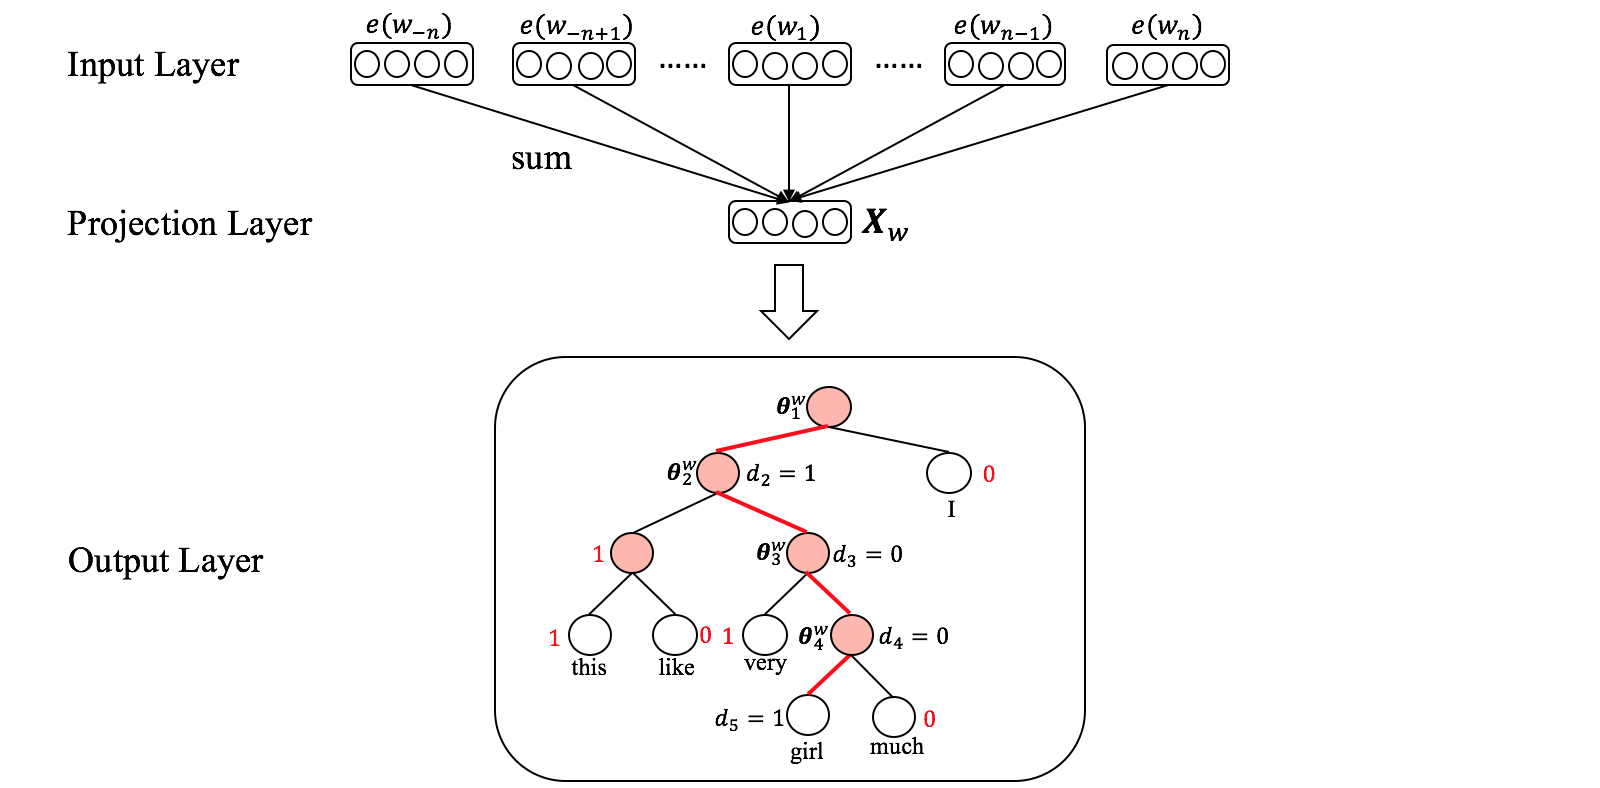
\includegraphics[width=\linewidth]{hierarchical_softmax.png}
    \bicaption{Hierarchical softmax模型}{Hierarchical softmax model}
    \label{fig:hierarchical_softmax}
\end{figure}
假设给定分类输入$\Vector{x}_w$,对任意一次二分类,分类到右分支称为正类,记作$d^w_i=1$,分类到左分支称为负类,记作$d^w_i=0$,则分类概率分别可定义为:
\begin{align}
    p_{right} &= \sigma(\Vector{x}_w^\mathrm{T}\theta) = \frac{1}{1+e^{-\Vector{x}^\mathrm{T}\theta}}\\
    p_{left} &= 1 - p_{right}
\end{align}
其中$\theta$就是需要训练的参数。于是,对于一个给定的词$w$,确定其关于上下文的条件概率的过程,就是根据该词的Huffman编码,得到其路径上每一次二分类分到该类$d^w_i$的概率,并将这些概率乘积:
\begin{equation}
    p(w|Context{w}) = \prod^{l(w)}_{j=2}p(d^w_j|\Vector{x}_w, \theta^w_{j-1})
\end{equation}
其中$l(w)$是$w$所在结点的深度。最后通过构建目标函数
\begin{equation}
\mathcal{L}(w,j) = (1-d^w_j)\log[\sigma(\Vector{x}_w^\mathrm{T}\theta^w_{j-1})] + d^w_j\log[1-\sigma (\Vector{x}_w^\mathrm{T}\theta^w_{j-1})]
\end{equation}
并调整参数使函数值最大化来训练模型。

当确定了$\theta$之后,模型也就确定了。同时在每一次更新参数的过程中,词$w$上下文窗口内的词向量也得到了更新:
\begin{equation}
    \Vector{v}(\tilde{w}) := \Vector{v}(\tilde{w}) + \eta\sum^{l{w}}_{j=2}\frac{\partial\mathcal{L}(w,j)}{\partial \Vector{x}_w}
\end{equation}
其中$\eta$为$w$对上下文词向量贡献的权重系数。

与CBOW相对的Skip-gram模型则在训练过程上十分类似,只是其模型投影层不再有加和等操作,而只把输入层的结果直接用来构造Huffman树。最后训练的过程则是求$p(Context(w)|w)$。具体就不再赘述。

上述过程称为基于Hierarchical Softmax的模型。为了简化训练过程,提高效率并且改善词向量的质量,Mikolov等人又采用Negative Sampling来对模型进行优化,避免了构建较为复杂的Huffman树。
以CBOW模型为例,其思想是指定一个关于当前词$w$的负样本集$NEG(w)$,采取下面的定义来获得词的正负类别标签,用来取代通过Huffam树获得的分类标签:
\begin{equation}
    L^w(\tilde{w}) = \left\{
        \begin{aligned}
            1, &\tilde{w} = w;\\
            0, &\tilde{w} \neq w;
        \end{aligned}
    \right.
\end{equation}
则给定训练样本$(Context(x), x)$,通过最大化
\begin{equation}
    g(w) = \prod_{u\in\{w\}\cup NEG{w}}p(u|Context(w))
\end{equation}
推导得到目标函数
\begin{equation}
    \mathcal{L} = \sum_{w\in C}\{\log[\sigma(\Vector{x}_w^\mathrm{T}\theta^w)] + \sum_{u\in NEG(w)}\log[\sigma(-\Vector{x}_w^\mathrm{T}\theta^u)\}
\end{equation}
用来训练模型参数。

\section{循环神经网络与长短时记忆网络}
\subsection{循环神经网络}
一般的神经网络模型中,就其数据流向而言,输入数据是单向传播的,即从输入层到输出层;就其网络结构而言,不同层之间的结点相互连接,但层内结点不存在连接。
这种网络结构在训练时独立看待每一次输入,其输出也是相互独立的;如果输入之间存在相互存在依赖或明显的相关关系,这些信息就很难学习得到。
但实际上,对于以序列形式存在的数据而言,如文本、语音等,这种情况是普遍存在的。

循环神经网络就是针对这类数据而提出的模型,它对序列化的数据有很好的适应性。
RNN的典型特征是,隐藏层中的神经单元存在到自身的连接,即在时域上展开之后,某时刻的结点也与其在前一时刻和后一时刻的状态相连。这样的结构使得模型能够在一定程度上记忆之前输入的信息,即序列中较早时刻输入的元素,也会对模型较晚时刻的输出产生影响。

\begin{figure}[H]
    \centering
    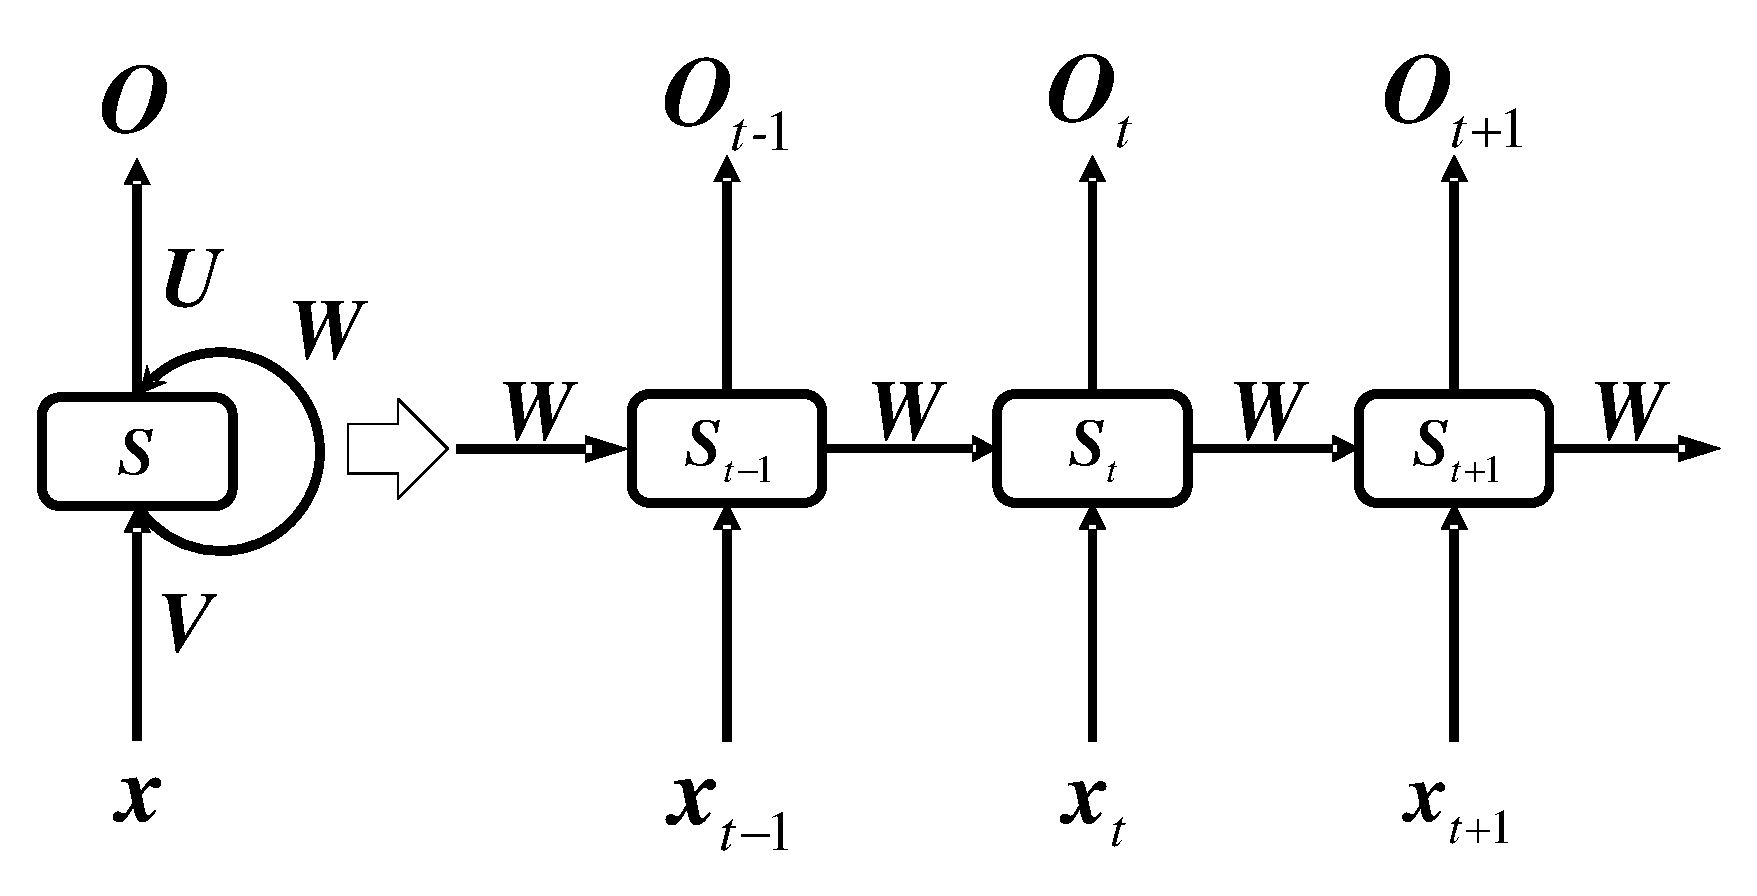
\includegraphics[width=0.8\textwidth]{RNN.pdf}
    \bicaption{RNN基本结构}{Basic RNN structrue}
    \label{fig:RNN}
\end{figure}

一个基本的RNN也可以看作包含输入层、单层隐藏层和输出层。
对于给定的输入序列$\Tensor{X}=\Vector{x}^n_0$,在每一个时刻,模型的输入是$\Vector{x}_t(t \in [0, 1, 2, \dots, n])$。隐层单元将按下式计算当前时刻的隐层状态和输出结果:
\begin{align}
    \Vector{s}_t &= f(\Matrix{U}\Vector{x}_t + \Matrix{W}\Vector{s}_{t-1})\\
    \Vector{o}_t &= g(\Matrix{V}\Vector{s}_t)
\end{align}
其中$\Vector{s}_t$是$t$时刻的隐层状态,即模型对序列信息保留的记忆;$\Matrix{U}$、$\Matrix{W}$、$\Matrix{V}$分别是输入层与隐层、隐层单元前后时刻和隐层与输出层之间的连接权重参数。
$f$、$g$是激活函数。

需要说明的是,一般而言我们在讨论RNN时提及的“带有单隐层的RNN”实际上指的是单层RNN单元在时域上展开,因此网络的深度与序列长度有关。
在这个过程中,$\Matrix{U}$、$\Matrix{W}$、$\Matrix{V}$的权重是共享的,即通过整个序列进行训练。
训练RNN的过程可转化为训练多层共享权重的前馈神经网络。
这里的“多层”指的就是RNN隐层在时域上展开后得到的深层神经网络。
训练时,正向计算目标函数后,反向传播误差时计算每一时刻上的误差,最后根据所有时刻上的导数更新权重。
这种算法称为Backpropagation through time(BPTT)。

但是在计算梯度时,由于序列长度可能很长,展开后的RNN层数可能很深,这样在计算时域上靠前的层的梯度时,就会产生多个导数相乘的形式,若其中存在多个值较小,那么其相乘的结果会迅速收敛到0,这就是“梯度消失”问题。

RNN普遍存在这种问题,从结果上看,这会导致RNN难以处理前后相隔较远的上下文依赖。一个简单的解决方案是替换激活函数,使用\verb|ReLu|替换\verb|sigmoid|或\verb|tanh|。而在RNN的基础上修改其单元的内部实现,比如使用长短时记忆模型(LSTM),则是更有效更普遍的方法。

\subsection{长短时记忆网络及其变体}
上文已经提及,虽然除$t_0$时刻的RNN单元外后续的每个单元接收的输入都带有之前所有时刻信息的累积,但受限于梯度消失问题,相隔较远的时刻输入对参数学习将不会有贡献,导致时域上靠后的单元无法很好地感知靠前的单元,句子内的长程依赖信息就无法被学习。

针对这一问题,S.Hochreiter和J.Schmidhuber\citep{hochreiter1997long} 在1997年提出了LSTM,其本质是使用带有信息存储和更新机制的单元代替RNN中相对较为简单的激活单元。信息存储即cell的内部状态,而更新机制则通过一系列“门控单元”实现,包括输入门、遗忘门和输出门。这些“门”会根据参数,对输入、cell状态和输出进行一系列处理,主要是对cell状态的更新进行控制,决定在状态上添加信息(记忆)还是减少信息(遗忘)。

一个基本的LSTM实现如图\ref{fig:LSTM}所示。其内部结构可描述为:
\begin{align}
\Vector{i}_t &= \sigma(\Matrix{W_i}\Vector{x}_t + \Matrix{U_i}\Vector{h}_{t-1} + \Vector{b}_i)
    \label{eq:lstm_i}\\
\Vector{f}_t &= \sigma(\Matrix{W_f}\Vector{x}_t + \Matrix{U}_f\Vector{h}_{t-1} + \Vector{b}_f)\\
    \Vector{o}_t &= \sigma(\Matrix{W}_o\Vector{x}_t + \Matrix{U}_o\Vector{h}_{t-1} + \Vector{b}_o)\\
    \Vector{a}_t &= \tanh(\Matrix{W}_C\Vector{x}_t + \Matrix{U}_C\Vector{h}_{t-1} + \Vector{b}_C)\\
    \Vector{C}_t &= \Vector{f}_t\odot\Vector{C}_{t-1} +
                    \Vector{i}_t\odot\Vector{a}_t
                    \label{eq:cell state}\\
    \Vector{h}_t &= \Vector{o}_t \odot \tanh(\Vector{C}_t)\label{eq:lstm_C}
\end{align}
其中$\odot$代表元素乘积,其结果仍是一个固定维度的实向量。

\begin{figure}[H]
    \centering
    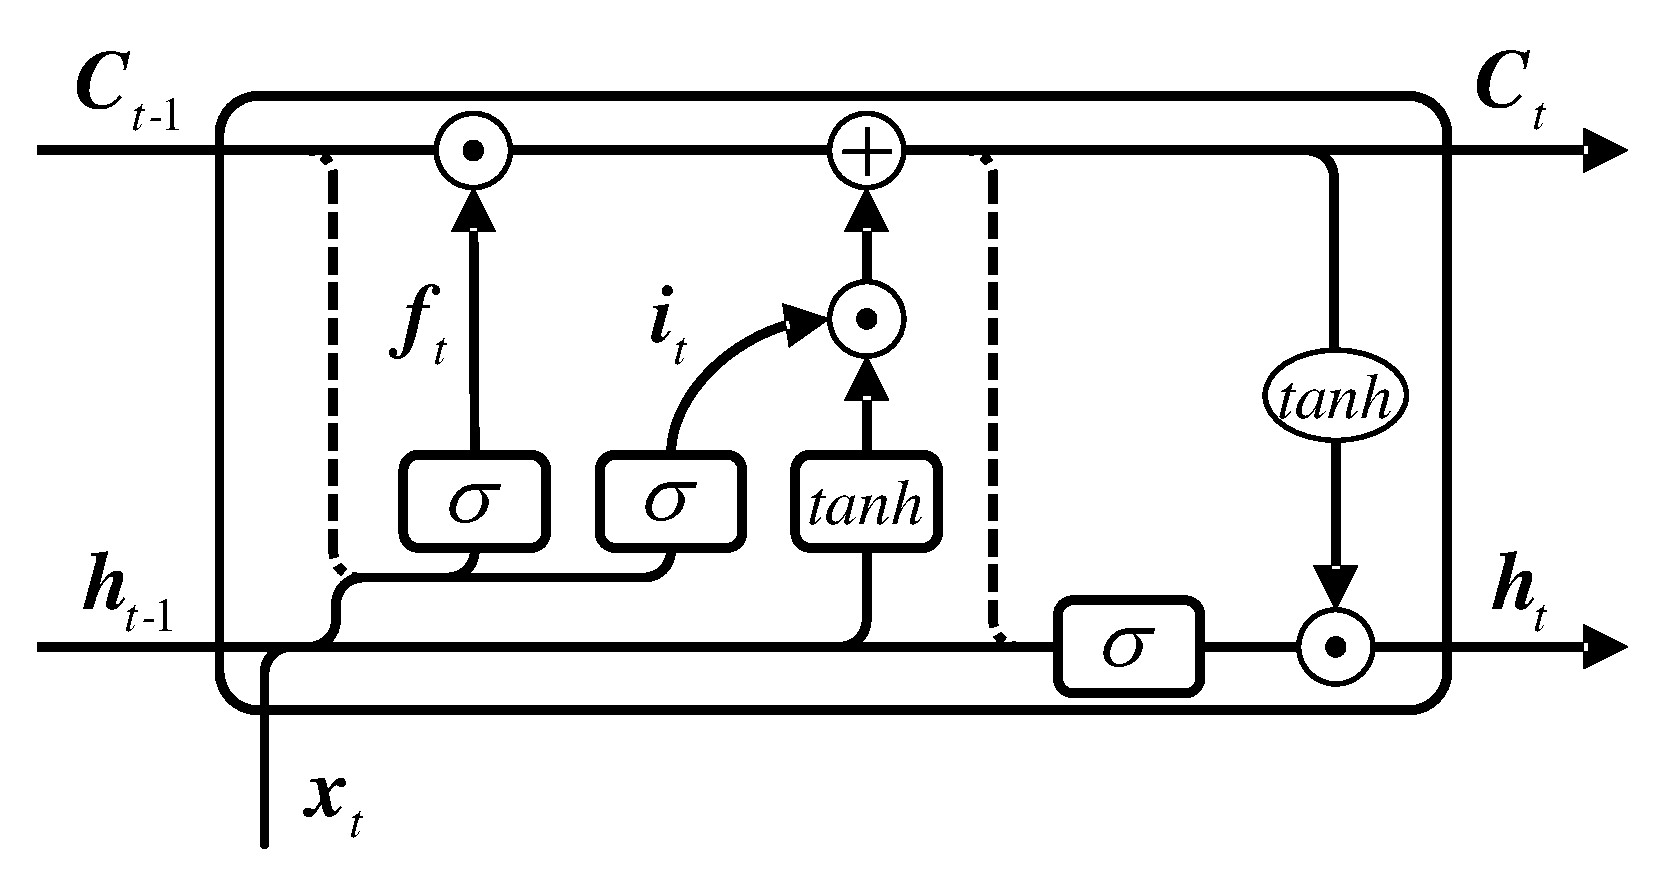
\includegraphics[width=0.8\textwidth]{LSTM-CIFG}
    \bicaption{LSTM的一般结构}{Common structure of LSTM}
    \label{fig:LSTM}
\end{figure}

首先,上一时刻的隐藏层状态$\Vector{h}_{t-1}$和当前时刻的输入词$\Vector{x}_t$经过连接构成了当前时刻的输入信息向量。这一向量将作为所有门控层\verb|sigmoid|激活函数的参数。

而经\verb|tanh|激活函数获得的激活值$\Vector{a}_t$则是一个临时的状态向量,其中包括了部分应该保留在cell状态中的信息,而其他信息则应该丢弃。

接着门控层根据模型参数和输入向量获得遗忘参数$\Vector{f}_t$和输入参数$\Vector{i}_t$。由式\ref{eq:cell state}可知,当前的cell状态将受到在输入门$\Vector{i}_t$控制下的临时状态向量$\Vector{a}_t$和在遗忘门$\Vector{f}_t$控之下的前一时刻cell状态$\Vector{C}_{t-1}$的共同影响。它们综合决定临时状态与历史状态中哪些信息应该得到保留,哪些信息应该丢弃。最终两部分保留的结果相加确定当前的cell状态。

为了更直观地观察到参数关系与维度,我们引入文献\citepns{arunmallyaLSTM}给出的形式来表示模型。在式\ref{eq:lstm_i}到\ref{eq:lstm_C}的基础上,设偏置向量$\Vector{b}*$整合进了$\Vector{x}_t$且:
\begin{align}
\hat{\Vector{i}}_t &= \Matrix{W}_i\Vector{x}_t + \Matrix{U}_i\Vector{h}_{t-1}\\
    \hat{\Vector{f}}_t &= \Matrix{W}_f\Vector{x}_t + \Matrix{U}_f\Vector{h}_{t-1}\\
    \hat{\Vector{o}}_t &= \Matrix{W}_o\Vector{x}_t + \Matrix{U}_o\Vector{h}_{t-1}\\
    \hat{\Vector{a}}_t &= \Matrix{W}_C\Vector{x}_t + \Matrix{U}_C\Vector{h}_{t-1}
\end{align}
则省略激活函数的情况下,参数可以组织为:
\begin{equation}
    \Vector{z}_t =
    \begin{bmatrix}
        \hat{\Vector{a}}_t\\
        \hat{\Vector{i}}_t\\
        \hat{\Vector{f}}_t\\
        \hat{\Vector{o}}_t\\
    \end{bmatrix}
    =
    \begin{bmatrix}
        \Matrix{W}_C & \Matrix{U}_C\\
        \Matrix{W}_i & \Matrix{U}_i\\
        \Matrix{W}_f & \Matrix{U}_f\\
        \Matrix{W}_o & \Matrix{U}_o\\
    \end{bmatrix}
    \times
    \begin{bmatrix}
        \Vector{x}_t\\
        \Vector{h}_{t-1}
    \end{bmatrix}
    =
    \begin{bmatrix}
        \Matrix{W}\times\Matrix{I}_t
    \end{bmatrix}
\end{equation}
若$x_t$为$n$维向量,隐层单元数为$m$,则$\hat{\Vector{a}}_t$,$\hat{\Vector{i}}_t$,$\hat{\Vector{f}}_t$,$\hat{\Vector{o}}_t$对应的权重矩阵$W*$、$U*$维数分别为$m\times n$、$m\times m$。
于是$W$的维数即为$4m\times(m+n)$。

上述基本的LSTM实现中,cell的历史状态$\Vector{C}_{t-1}$并不能影响遗忘门$\Vector{f}_t$和输入门$\Vector{i}_t$对临时状态$\Vector{a}$和自身信息是否保留的决策。
因此文献\citep{sak2014long}给出了LSTM cell的一个改进版本,它在原有LSTM定义的输入向量上扩展了历史cell状态的部分,即在进行遗忘/保留决策时,还需要考虑到历史记忆。
这一机制称为peep-hole,即在图\ref{fig:LSTM}所示LSTM结构基础上增加虚线部分。
其内部参数可表示为:
\begin{align}
    \Vector{i}_t &= \sigma(\Matrix{W}_{i}\Vector{x}_{t} + \Matrix{W}_{i}\Vector{h}_{t-1} + \Matrix{W}_{i}\Vector{C}_{t-1} + \Vector{b}_i)\\
    \Vector{f}_t &= \sigma(\Matrix{W}_{f}\Vector{x}_{t} + \Matrix{W}_{f}\Vector{h}_{t-1} + \Matrix{W}_{f}\Vector{C}_{t-1} + \Vector{b}_f)\\
    \Vector{o}_t &= \sigma(\Matrix{W}_{o}\Vector{x}_{t} + \Matrix{W}_{o}\Vector{h}_{t-1} + \Matrix{W}_{o}\Vector{C}_{t-1} + \Vector{b}_o)\\
    \Vector{a}_t &= \tanh(\Matrix{W}_{C}\Vector{x}_t + \Matrix{W}_{C}\Vector{h}_{t-1} + \Vector{b}_{C})\\
    \Vector{C}_t &= \Vector{f}_t\odot\Vector{C}_{t-1} + \Vector{i}_t\odot \Vector{a}_t \\
    \Vector{h}_t &= \Vector{o}_t \odot \tanh(\Vector{C}_t)
\end{align}
在上述使用peep-hole的LSTM cell的基础上,文献\citep{lample2016neural}在命名实体识别任务上还使用了耦合输入-遗忘门(Coupled Input-Forget Gate, CIFG)取得了较好的效果,即令
\begin{equation}
    \Vector{f}_t = 1 - \Vector{i}_t
\end{equation}
对比LSTM cell简化了CIFG的计算:
\begin{equation}
    \Vector{C}_t = (1 - \Vector{i}_t)\odot \Vector{C}_{t-1} + \Vector{i}_t\odot \tanh(\Matrix{W}_{Cx}\Vector{x}_t + \Matrix{W}_{ch}\Vector{h}_{t-1} + \Vector{b}_C)
\end{equation}

文献\citep{cho2014learning}提出了一种更为简单的LSTM单元的变体,称为门控循环单元(Gated Recurrent Unit,GRU)。
GRU存在多种变体,区别在于计算每个门层输出是否使用之前的隐藏状态和偏置。
本节仅介绍使用隐藏状态计算门层输出的GRU,如图\ref{fig:GRU}所示。
其最主要的特征是
\begin{enumerate}
    \item 融合了cell状态和隐藏层输出
    \item 融合了输入门和遗忘门
\end{enumerate}

\begin{figure}[H]
    \centering
    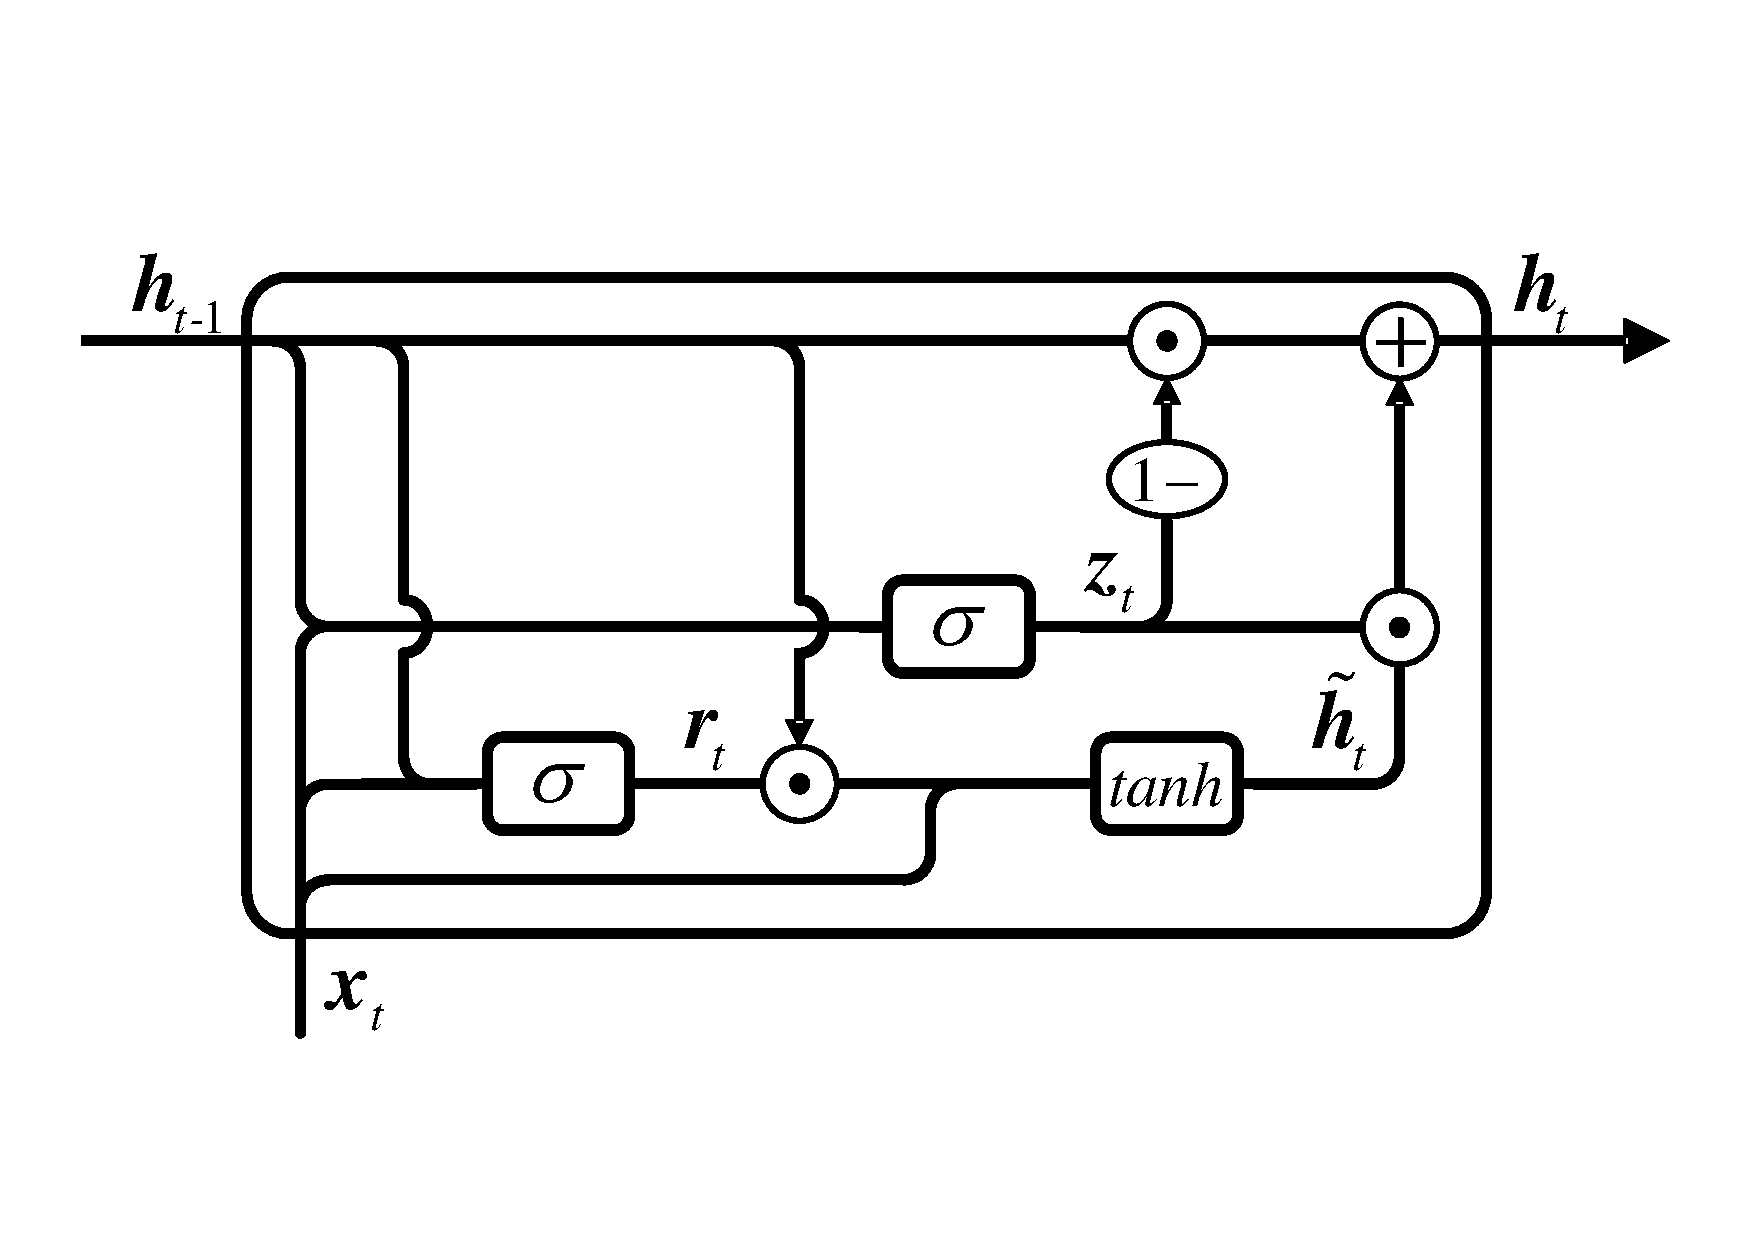
\includegraphics[width=0.8\linewidth]{GRU}
    \bicaption{GRU基本结构}{Basic structure of GRU}
    \label{fig:GRU}
\end{figure}
这使得单元相比LSTM更加简单,参数更少,同时实验表明它能够在大部分任务中取得与LSTM相当或更佳的效果。
其内部参数可表示为:
\begin{align}
    \Vector{z}_t &= \sigma(\Matrix{W}_{z}\Vector{x}_t + \Matrix{W}_{z}\Vector{h}_{t-1})\\
    \Vector{r}_t &= \sigma(\Matrix{W}_{r}\Vector{x}_t + \Matrix{W}_{r}\Vector{h}_{t-1})\\
    \Vector{\tilde{h_t}} &= \tanh(\Matrix{W_{\tilde{h}u}}(\Vector{r}_t \odot \Vector{h}_{t-1}) + \Matrix{W_{\tilde{h}x}}\Vector{x}_t)\\
    \Vector{h}_t &= (1 - \Vector{z}_t) \odot \Vector{h}_{t-1} + \Vector{z}_t \odot \Vector{\tilde{h}}_t
\end{align}

LSTM存在很多种变体,也有文献系统地对比了多种变体在自然语言处理任务上的性能。本文也将在具体的场景下,对比分析不同的结构对命名实体识别效果的影响。

\section{双向LSTM-CRF序列标注框架}
\subsection{双向LSTM层}
回顾一下从语言模型和传统的命名实体识别方法到神经语言模型和长短时记忆模型,我们可以发现语言模型从统计字/词共现频数估计序列的条件概率,经典的HMM在马尔可夫假设下估计作为隐藏状态的标签转移概率,神经语言模型同样也是根据上文序列推导下文词语的条件概率。
这些模型和方法在形式上都有着一个共同的特点,即尽可能地利用上文信息来进行训练和预测。

在序列标注任务下,具体如命名实体识别任务下,真实语境中的命名实体完全可能在语义和语法上同时依赖上下文。如何同时有效地利用待识别序列上下文的信息,这就给模型提出了新的要求。

在序列正向输入到LSTM中时,LSTM能够很好地“记忆”上文的信息,一个自然的想法是,如果想获取下文的信息,是否可以将序列逆序输入LSTM以达到这个目的。
文献\citep{huang2015bidirectional, ma2016end}等已经指出,通过两个结构相同、参数独立的LSTM层分别接受正序、逆序的输入序列,能够较好地同时获取上下文的依赖信息。

\begin{figure}[H]
    \centering
    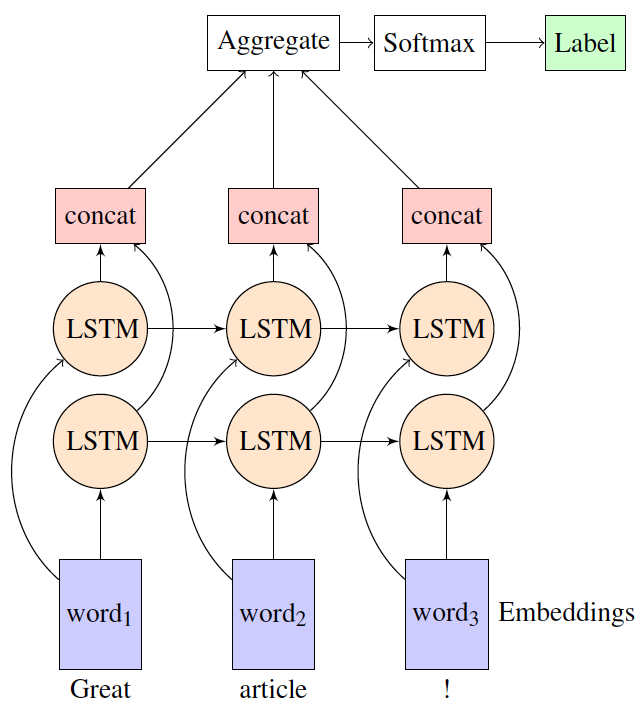
\includegraphics[width=0.6\textwidth]{BiLSTM.png}
    \bicaption{双向LSTM结构}{Structure of bi-directional LSTM}
    \label{fig:BiLSTM}
\end{figure}

基于双向LSTM-CRF框架的序列标注框架已经在各项序列标注任务上取得了很好的成果,这一方法由于较少依赖人工特征,能够实现端到端的标注,因此在使用神经网络方法的序列标注任务上,该框架已经成为了主流的方法。
具体地,如图\ref{fig:BiLSTM}所示就是一个使用双向LSTM的标注框架。
其中使用了两层方向不同的LSTM层,对于$t$时刻的输入词向量分别在两层LSTM获得输出$\overrightarrow{\Vector{h}}_t$和$\overleftarrow{\Vector{h}}_t$,分别代表保留了上文信息和下文信息的隐层状态。
可以对这两层输出进行连接或加和等操作,获得最终的隐层输出。

最后,一般在输出层进行一次\verb|Softmax|,用来进行一次维度转换,将由两层LSTM获得的包含上下文信息的词特征向量,映射到维度为标签数目的空间中。
如果单纯使用LSTM做序列标注,则这时的输出就可以理解为当前词属于某标签类别的概率。
最简单的可以取每个时刻输出的最大值对应的标签,这样就获得了由LSTM标注的标签序列。
\subsection{CRF层}
\subsubsection{为什么要使用CRF层}
除了上下文的信息,对自然语言序列标注还需要结合实际的语言习惯和语法规则。
这些语法规则表现在标注输出标签之间存在较强的依赖性。
以\verb|BIO|标注体系标注命名实体为例,基本元素为字符,\verb|B|为命名实体起始字,\verb|I|为命名实体中间字,\verb|O|为非命名实体字。
则标签\verb|I|不应该独立出现,其前面的标签应该为\verb|B|或\verb|I|;而就类别而言,表示人名起始字的\verb|B-PER|后也不应该出现表示地名的中间字标签\verb|I-LOC|。
上一节提到,单纯使用LSTM做序列标注时,若简单地选取每一时刻输出的最大概率值对应的标签来构建标签序列的话,就无法考虑这些规则。
这样就会存在许多输出序列不符合这类规则,影响标注结果。

借用节\ref{chap:HMM}中提到的概念,我们可以理解为:LSTM很好地学习到了作为观察序列的文本的上下文信息,但不能学习到作为隐藏状态的标签的前后约束关系;
CRF可以很好地学习到标签之间的转移权重(与转移特征函数相关的部分),但其状态特征函数部分,即给定序列获取当前位置标签的概率的部分较难定义,需要依靠人工特征等来建立,而这一部分LSTM能够得出理想结果。
因此结合双向LSTM-CRF显然是合理的选择。
\subsubsection{CRF层的工作原理}
本节将简单介绍BiLSTM-CRF框架在CRF层中的参数与训练过程。

给定输入序列
\begin{equation}
    \Vector{X} = [\Vector{x}_1, \Vector{x}_2,\dots, \Vector{x}_n]
\end{equation}
LSTM层在时刻$t$对输入$\Vector{x}_t$的输出为预测$\Vector{x}_t$标签的概率分布向量$\Vector{d}_t$。
则对整个输入序列$\Vector{X}$,LSTM层输出为
\begin{equation}
    \Matrix{P} = [\Vector{d}_1,\Vector{d}_1,\dots,\Vector{d}_n]
\end{equation}
$\Matrix{P}$为$n\times k$矩阵,$k$为标签类别数。
则$\Matrix{P}_{i, j}$表示第$i$个输入是标签$j$的概率。对于一个可能的预测结果序列
\begin{equation}
    \Vector{y}=(y_1, y_2,\dots, y_n)
\end{equation}
其中$y_t$是$t$时刻的预测标签索引。可定义该预测序列在给定输入序列下的评分:
\begin{equation}
    s(\Vector{X},\Vector{y})=\sum^n_{i=0}\Matrix{A}_{y_i,y_{i+1}}+\sum^n_{i=1}P_{i, y_i}
\end{equation}
其中$\Matrix{A}$为转移矩阵,即$\Matrix{A}_{i,j}$为标签$i$到标签$j$的转移概率,矩阵$\Matrix{A}$就是CRF层需要学习的参数。
转移概率中可以学习到标签之间存在的约束。序列$\Vector{y}$实际上是在矩阵$\Matrix{P}$中按照时间顺序选择的一条路径。
序列概率可由\verb|Softmax|函数计算:
\begin{equation}
    p(\Vector{y}|\Vector{X})=\frac{\exp\{s(\Matrix{X},\Vector{y})\}}{\sum_{\tilde{\Vector{y}}\in Y_{\Matrix{X}}}\exp\{s(\Matrix{X},\tilde{\Vector{y}})\}}
\end{equation}
其中$Y_{\Matrix{X}}$是对于输入序列$\Matrix{X}$所有可能出现的预测序列观测值集合。
若序列$\Vector{y}$是正确的预测结果序列,则在训练过程中需要最大化该序列的对数概率
\begin{equation}
    \log(p(\Vector{y}|\Matrix{X})) = s(\Matrix{X},\Vector{y})-\log(\sum_{\tilde{\Vector{y}}\in Y_{\Matrix{X}}}\exp\{s(\Matrix{X},\tilde{\Vector{y}})\})
\end{equation}

预测过程中,选择预测结果$\Vector{y}*$使得其序列评分最高即可
\begin{equation}
    \Vector{y*}=\mathop{\arg\max}_{\tilde{\Vector{y}}\in Y_{\Matrix{X}}} s(\Matrix{X},\Vector{\tilde{y}})
\end{equation}
\section{模型训练与参数调优}
\subsection{批量训练}
在训练过程中,每输入一定量的训练数据训练模型后,就要对模型参数进行更新。
参数更新需要根据优化算法计算得到的梯度结果进行。
优化算法有很多种,包括随机梯度下降(Stochastic Gradient Descent, SGD)、Momentum、Adadelta、Rmsprop等等。
本质上都是策略不同的梯度下降算法。

以SGD为例,更新参数的时机有两种极端的选择,一种是对每一条训练数据进行一次参数更新,这种策略就是原始的stochastic gradient descent。
该策略计算速度快,但对于每个数据样本,其能够产生的梯度方向都可能不同,不同的数据样本对参数的更新又可能相互抵消,造成训练震荡,这就导致模型较难收敛到最优点。
另一种是对所有的训练数据更新一次参数,这种策略内存占用多,计算资源消耗大,但其参数的更新依据的是全样本的特征,获得最优结果相对容易,但选取合适的学习率很难。

一个折衷的方案就是选取一个合适的数据规模,即批尺寸(batch-size),来使用一批规模相对较小的数据来更新参数。这样的一批参数称为mini-batch。
梯度采用这一批数据的平均梯度,参数的更新由这一批数据共同影响。一定程度上,这种更新策略减少了梯度下降的随机性,同时也减少了计算资源的开销。
\subsection{防止过拟合}
在深度学习中,防止过拟合的方法有很多种。本文主要应用了以下三种,下面进行简单介绍。
\subsubsection{正则化}
正则化即在计算目标函数时增加相应参数的正则化项。

设模型参数为$w_i^n$,则L1正则化项为:
\begin{equation}
    L_1 = \sum^n_{i=1}\lVert w_i \rVert_1
\end{equation}

L2正则化项为:
\begin{equation}
    L_2 = \sum^n_{i=1}\lVert w_i \rVert_2^2
\end{equation}

正则化项可以加在输入层、LSTM(包括偏置项)权重参数上。在优化目标函数时,同时也要考虑正则化参数的值,使模型在训练时尽量趋于简单,减少对不必要数据的拟合。
\subsubsection{Dropout}
Hinton在文献\citep{srivastava2014dropout}中提出了Dropout方法防止过拟合。其基本思想是神经网络在拟合一个模型的时候,神经元之间会产生复杂的共同适应性。但神经元在训练时不应依赖其他特定的神经元,因此需要随机去除一些神经元,使得网络结构看起来像是随机生成的,训练过程类似是对多种不同的神经网络训练结果进行了综合,由于不同网络过拟合的方式不同,因此综合不同网络的结果在一定程度上可以消除这些过拟合。在实现中的做法是,随机根据给定的概率忽略掉部分神经元,被忽略掉的神经元的输出为0。这样做可以增强模型的鲁棒性,减少过拟合情况,但同时也会增加训练的时间。

对LSTM使用dropout时,主要针对输入层和输出层进行dropout。
\subsubsection{Early stopping}
早停机制(Early stopping)即在训练模型过程中同步评估模型误差,当模型误差不再降低时,停止训练。

实际操作中,我们一般将数据集分为训练集、验证集、测试集。其中训练集用于训练模型,验证集用于在训练过程中定期测试模型误差。
训练过程中,随着模型对数据充分地学习,其在训练集、验证集上的误差应该同步下降;当模型在训练集上的误差继续下降,但在验证集上的误差不再下降时,模型就有过拟合的可能。
这时及时停止训练,可以避免模型过拟合。
\section{本章小结}
本章首先从词的分布式表示入手,介绍了词向量、神经网络语言模型,着重讨论了基于Hierarchical Softmax的词向量生成过程。
然后,对RNN的网络结构进行了介绍,对比分析了LSTM及其多种变体的实现差异。
接着讨论了双向LSTM-CRF序列标注框架结构,并分析了CRF层在该框架中的具体作用和训练方法。
最后,针对模型训练过程中常采用的参数更新策略和防止过拟合方法进行了简单介绍。
本文拟通过本章介绍的序列标注框架实现命名实体识别的基线模型,并在不同任务场景下进行实验,比较其与其他方法在性能上的差异。

